\thispagestyle{empty}
\underline{~~~~~~~~~~~~~~~~~~~~~~~~~~~~~~~~~~~~~~~~~~~~~~~~~~~~~~~~~~~~~~~~~\huge 4 \hspace{8cm}}
\begin{center}
\tiny A Н Д Р Е Й\quad  Н И К О Л А Е В И Ч\quad   К О Л М О Г О Р О В
\end{center}
\begin{multicols}{2}
\begin{tikzpicture}[>=stealth] 
\draw[->, thin] (-3,0) -- (3.3,0)node[below] {$x$};  
\draw[->, thin] (0,-3) -- (0,3.3)node[left] {$y$};  
\draw[thick] (2.5,0) arc (0:180:2.5);
\node[below left] at (0,0) {$O$};
\draw[dashed, thick] (2.5,0) arc (0:-180:2.5);
\node[below left] at (-2.5,0) {$-1$};
\node[below right] at (2.5,0) {$1$}; 
\draw[thick,dashed,] (-1,0) -- (-1,2.3) --(0,2.3);
\node[below left] at (0,3) {$1$}; 
\draw[dashed, thick] (2.3,0) -- (2.3,1)--(0,1);
\node[below left] at (0,-2.5) {$-1$}; 
\draw (2.3,1) circle (0.06cm);
\draw (-1,2.3) circle (0.06cm);
\end{tikzpicture}

\noindentдем считать знаком извлечения арифметического квадратного корня. Равенство 
\[y = \sqrt{1-x}\eqno{\rm (1)}\]
обозначает, что выполнены условия 
\[x^2 \leq 1,~ y \geq 0, ~ x^2 + y^2 = 1\eqno{\rm (2)}\]

Точки, координаты которых удовлетворяют этим условиям, образуют полуокружность, изображенную на рисунке 1.

Рисунок 1 делает наглядными следующие факты, которые вы можете доказать и чисто алгебраическим путем:

1) формула (1) позволяет для любого х, удовлетворяющего условиям
\[-1 \leq x \leq 1,\eqno{\rm (3)}\]
вычислить соответствующее ему у, которое удовлетворяет неравенствам
\[0 \leq y \leq 1;\eqno{\rm (4)}\]

2) каждому у, удовлетворяющему неравенствам (4), соответствует хотя бы одно такое х, которому по формуле (1) соответствует это заданное у.

Можно сказать, что формула (1) задает отображение множества чисел х, удовлетворяющих неравенствам (3), на множество чисел, подчиненных неравенствам (4). Математики часто (особенно в последнее время) для обозначения отображений употребляют стрелку. Занимающуее нас отображение можно записать при помощи стрелки так:
\[x \rightarrow \sqrt{1 - x^2}\eqno{\rm (5)}\]

Заметьте: \textit{ображение полностью определено, если а) задано множество Е, которое отображается; 6) для каждого элемен-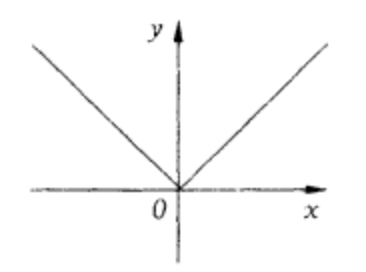
\includegraphics[width=0.7 \linewidth]{2pic}\\
\[\scriptsize\text{Рисунок 2}\] та х этого множества В задан элемент у, на который элемент х отображается.}


Множество всех значений у обозначим буквой М. В первом примере Е — множество чисел, удовлетворяющих условию (3), а М — множество чисел, удовлетворяющих условию (4).

\textbf{Пример 2.} Правила\\
1)\(x \rightarrow \sqrt{x^2},\)\\
\hfill \break
2)\( x \rightarrow
  \begin{cases}
     x, & \quad \text{если } x \geq 0,\\
    -x,  & \quad \text{если } x < 0
  \end{cases}
\)\\
определяют одно и то же отображение
\[x \rightarrow |x|\eqno{\rm (6)}\]
действительных чисел х на их модуди (абсолютные величины) (рис. 2).

Отображение (6) отображает множество всех действительных чисел
\[R =(-\infty; +\infty)\]
на множество
\[R_+ =[0; +\infty)\]
неотрицательных действительных чисел,

Вместо слова \textit{отображение} можно говорить \textit{функция} и записать отображение (5) так:
\[f(x) = \sqrt{1 - x^2}\eqno{\rm (7)}\]
а отображение (6) так:
\[f(x) = |x|\eqno{\rm (8)}\]

Областью опрелеления функции (8) является множество всех действительных чисел R. Множеством ее значений является множество \(R_+\), неотрицательных действительных чисел.

\textbf{Пример 3.} Петя, Коля, Саша и Володя живут в комнате общежития. На февраль
они установили такой график дежурств:\\
\begin{tabular}{ | l | l | l | l | l | l |l | l | l | l | l | l |l | l |}
\hline
& 1& 2& 3& 4& 5& 6& 7& 8& 9& 10& 11& ... & 28\\ \hline
Петя& \cellcolor{black}& & & & \cellcolor{black}& & & & \cellcolor{black}& & & &\\ \hline
Коля& & \cellcolor{black}& & & & \cellcolor{black}& & & & \cellcolor{black}& & &\\ \hline
Саша& & & \cellcolor{black}& & & & \cellcolor{black}& & & & \cellcolor{black}& &\\ \hline
Володя& & & & \cellcolor{black}& & & & \cellcolor{black}& & & &  &\cellcolor{black}\\ \hline
\end{tabular}

\end{multicols}
\thispagestyle{empty}